\section{Results}

We evaluate Q-learning (QL), model-based RL (MBRL) and Floyd-Warshall
Reinforcement Learning (FWRL) on two metrics in two different environments. The
two metrics we use are Latency Ratio and average reward per episode. The Latency
ratio metric was introduced in \citet{MiPaViICLR2017}, which is defined as the
ratio of time taken to reach the goal for the first to time to the average time
taken to hit the goal thereafter. The Latency ratio thus measures the ratio of
exploration time for first time finding the goal to the average exploitation
time to reach the goal. Hence, higher latency ratio is better.
Fig~\ref{fig:ql-fw-grid-world-results} and
Fig~\ref{fig:ql-fw-windy-world-results} show the results.

\begin{figure}%
    \begin{minipage}{\columnwidth}
        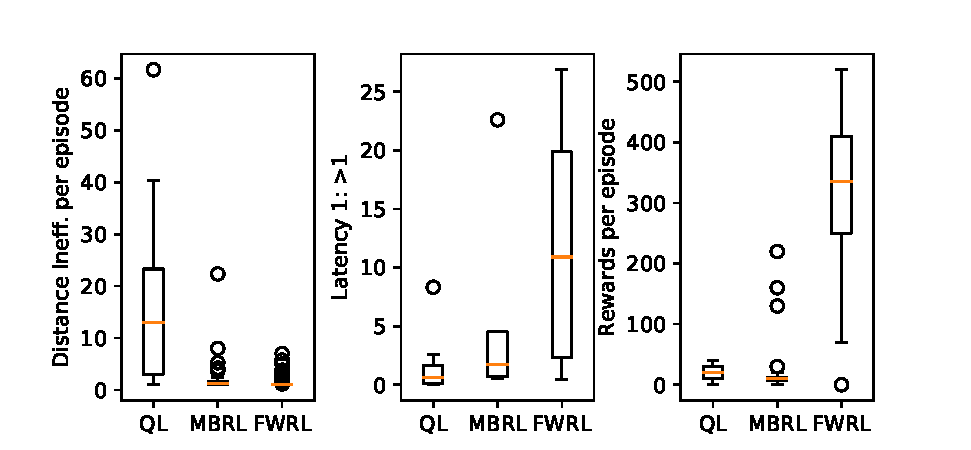
\includegraphics[width=\columnwidth]{./media/metrics-grid-world.pdf}{a}
        \caption{Results on grid world. FWRL beats Q-Learning
        consistently. Lower is better for Distance-Inefficiency. Higher
        is better for reward per episode. }
      \label{fig:ql-fw-grid-world-results}%
    \end{minipage}
    \begin{minipage}{\columnwidth}
        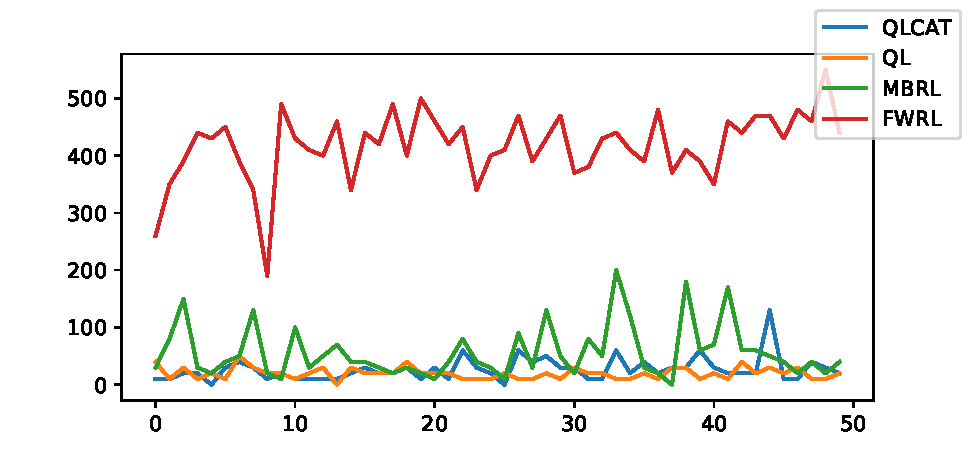
\includegraphics[width=\columnwidth]{./media/rewards-metrics-grid-world.pdf}{b}
        \caption{Reward curves on grid world. FWRL reward climbs much
        faster than all other baselines showcasing the improved \emph{sample
        efficiency} of the algorithm.}
      \label{fig:ql-fw-grid-world-reward-curves}%
    \end{minipage}
\end{figure}


\begin{figure}
    \begin{minipage}{\columnwidth}
        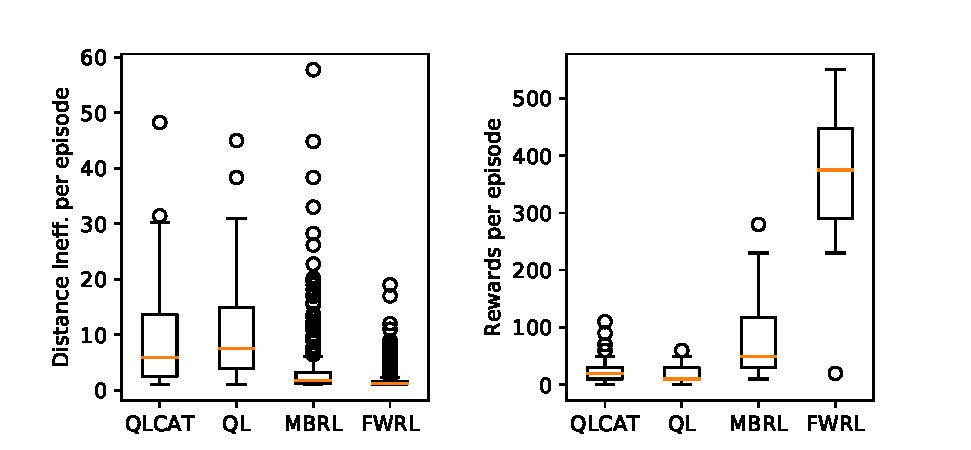
\includegraphics[width=\columnwidth]{./media/metrics-windy-world.pdf}
        \caption{Results on windy world. FWRL beats Q-Learning
        consistently. Lower is better for Distance-Inefficiency. Higher
        is better for reward per episode. }
      \label{fig:ql-fw-windy-world-results}%
    \end{minipage}
    \begin{minipage}{\columnwidth}
        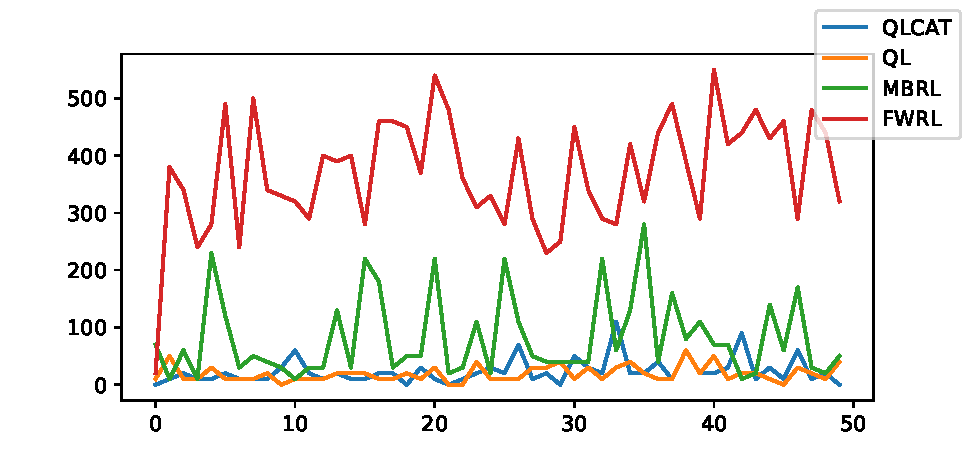
\includegraphics[width=\columnwidth]{./media/rewards-metrics-windy-world.pdf}
        \caption{Reward curves on windy world. FWRL reward climbs much
        faster than all other baselines showcasing the improved \emph{sample
        efficiency} of the algorithm.}
    \label{fig:ql-fw-windy-world-reward-curves}%
    \end{minipage}
\end{figure}


\subsection{Qualitative Results}

To demonstrate the claim made in Fig~\ref{fig:visual-abstract}, we train QLCAT
and FWRL for two episodes each with start and goal locations such that the path
meets in the center. Unlike quantitative experiments, in this experiment the
episode ends when the agent reaches the goal.
After two episodes of training, in which both FWRL (Floyd-Warshall RL) and QLCAT
(Q-Learning with goal concatenated to the state) reach the desired
goals via exploration, we put the algorithms to test.
For the test episode, the goal is chosen from first training episode but start
location is chosen from second training episode.
During the test episode,
we turn off $\epsilon$-greed exploration and follow the greedy policy.

We find that QLCAT decides to repeat the action that pushes it into the wall,
therefore is unable to move. However, FWRL reaches the goal using the shortest
path. The trajectories and value functions are visualized in Figure~\ref{fig:qualitative-results}.

\begin{figure}
  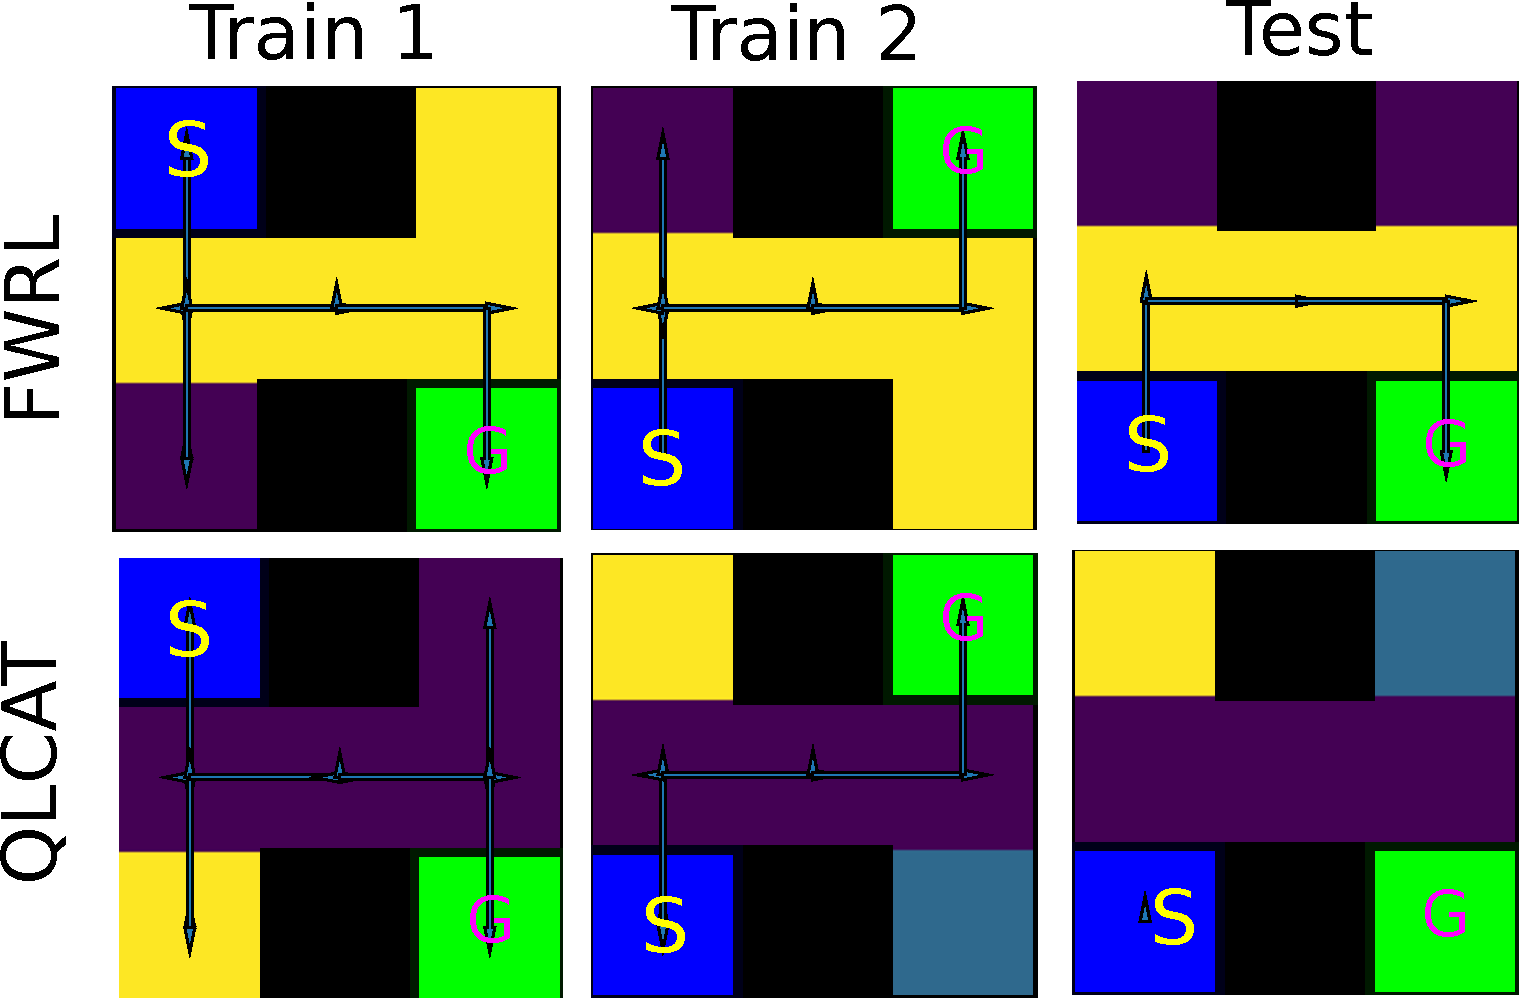
\includegraphics[width=\columnwidth]{./media/qualitative-results.pdf}
  \caption{Qualitative results: Visualization of value-function in H-Maze. Green
box with G represents goal location, Blue box with S represents start location.
The obstacles are shown black. The trajectories are shown by arrows. The color
of remaining boxes show the expected value of each state computed by the
corresponding algorithm. Each row different algorithm, while columns show
different episodes. We find that QLCAT is unable to learn a new trajectory
when given an unseen combination of start and end location. FWRL (ours) finds the
shortest path easily in such a test case. }
\label{fig:qualitative-results}
\end{figure}
